\documentclass[12pt,a4paper]{article}

\usepackage{listings}
\usepackage{xcolor}
\usepackage{graphicx}

\definecolor{codegreen}{rgb}{0,0.6,0}
\definecolor{codegray}{rgb}{0.5,0.5,0.5}
\definecolor{codepurple}{rgb}{0.58,0,0.82}
\definecolor{backcolour}{rgb}{0.95,0.95,0.92}

\lstdefinestyle{mystyle}{
	backgroundcolor=\color{backcolour},   
	commentstyle=\color{codegreen},
	keywordstyle=\color{magenta},
	numberstyle=\tiny\color{codegray},
	stringstyle=\color{codepurple},
	basicstyle=\footnotesize,
	breakatwhitespace=false,         
	breaklines=true,                 
	captionpos=b,                    
	keepspaces=true,                 
	numbers=left,                    
	numbersep=5pt,                  
	showspaces=false,                
	showstringspaces=false,
	showtabs=false,                  
	tabsize=2
}
\lstset{style=mystyle}


\title{Problem Set 1 - Solution}
\date{Due: October 1, 2021}
\author{Dino Wildi}

\begin{document}

\maketitle

\section{Question 1: Education}

\subsection{Task 1}
\textit{A school counselor was curious about the average of IQ of the students in her school and took a random sample of 25 students' IQ scores. The following is the data set:\\}
\vspace{.5cm}
\lstinputlisting[language=R, firstline=40, lastline=40]{PS01.R}  
\vspace{0.5cm}

In the data provided by the school counselor, we have a sample size of n = 25; this is not enough to use a normal distribution. Hence, I am using a t-distribution to account for the small sample size. In R, I am using the qt() command to find the t-score for the given data and multiply it with the estimated standard deviation to get the appropriate margin of error. I am then subtracting and adding that margin to the mean of the sample to find the bounds of the confidence interval:

\lstinputlisting[language=R, firstline=15, lastline=18]{PS01_DW_R.R}

According to this calculation, the confidence interval at the significance level alpha = 90\% is \textbf{[93.960, 102.920]}, with the estimated mean being \textbf{98.44}.

\subsection{Task 2}
\textit{Next, the school counselor was curious  whether  the average student IQ in her school is higher than the average IQ score (100) among all the schools in the country. Using the same sample, conduct the appropriate hypothesis test with $\alpha=0.05$.}
\vspace{0.5cm}

The second question asks for a hypothesis test for the hypothesis that the mean level of intelligence at the school is higher than the average intelligence level in the country, which is stated to be 100. Formally speaking, the alternative hypothesis and the corresponding null hypothesis read:

\[HA: \mu > 100\]\[H0: \mu \leq 100\]

We try to reject the null hypothesis with a one-sided t-test, with the alternative hypothesis being specified as “greater” according to the direction of the sign in HA. The confidence level we are specifying is 95\%, i.e. we seek a p-value below 0.05.

\lstinputlisting[language=R, firstline=23, lastline=23]{PS01_DW_R.R}

The results of the t-test are clearly not sufficient to reject the null hypothesis. The estimated mean is \textbf{98.44}, below the hypothesised mean of 100. The p-value for the null hypothesis is \textbf{0.72}, far above the specified confidence level of p = 0.05. We have to assume that the true mean intelligence of students at the counselor’s school is not above 100.\pagebreak

\section{Question 2: Political Economy}

\textit{Researchers are curious about what affects the amount of money communities spend on addressing homelessness. The following variables constitute our data set about social welfare expenditures in the USA.} \\
\vspace{.5cm}

\begin{tabular}{r|l}
	\texttt{State} &\emph{50 states in US} \\
	\texttt{Y} & \emph{per capita expenditure on shelters/housing assistance in state}\\
	\texttt{X1} &\emph{per capita personal income in state} \\
	\texttt{X2} &  \emph{Number of residents per 100,000 that are "financially insecure" in state}\\
	\texttt{X3} &  \emph{Number of people per thousand residing in urban areas in state} \\
	\texttt{Region} &  \emph{1=Northeast, 2= North Central, 3= South, 4=West} \\
\end{tabular}

\vspace{.5cm}
\textit{Explore the \texttt{expenditure} data set and import data into \texttt{R}.}
\vspace{.5cm}

\lstinputlisting[language=R, firstline=30, lastline=30]{PS01_DW_R.R}


\subsection{Task 1}
\textit{Please plot the relationships among \emph{Y}, \emph{X1}, \emph{X2}, and \emph{X3}? What are the correlations among them (you just need to describe the graph and the relationships among them)?}
\vspace{0.5cm}

The first task asks for the associations between Y and the three X-variables given in the expenditure dataset. I have created the six plots for all respective associations using ggplot, both with a scatterplot and a line delineating the association of the two variables in each individual plot. The results are represented in Figure \ref{fig:refplot}, with the top row representing the individual associations between Y and each X; the bottom row represents the correlations of the individual X variables.

\lstinputlisting[language=R, firstline=34, lastline=48]{PS01_DW_R.R}

\begin{figure}[h]
	\centering
	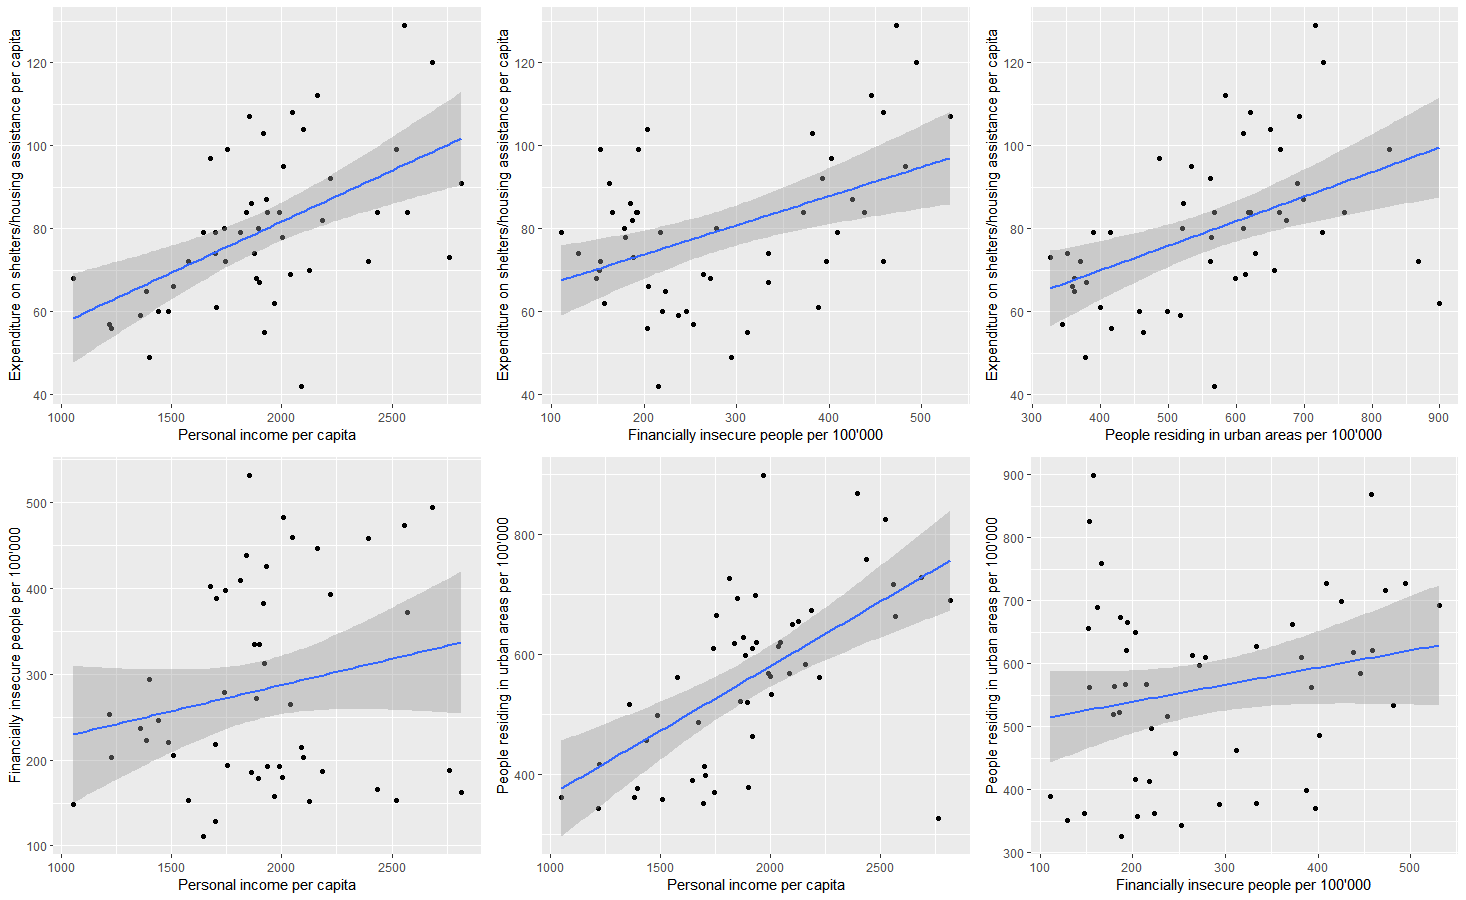
\includegraphics[width=\textwidth]{PS1_Plot1}
	\caption{Relations between Y, X1, X2, and X3}
	\label{fig:refplot}
\end{figure}

In the top row, we can observe a positive correlation between the expenditure per capita on shelters and housing assistance (i.e. Y) and each individual X. The effect is largest for X1, personal income per capita. The confidence intervals plotted alongside the regression line also indicate that the effect is unlikely to be purely random, as they are relatively narrow alongside the regression line.

In the bottom row, we see three plots outlining the correlations between individual explanatory variables. Here, we would ideally observe no correlations whatsoever. However, we see a strong association between personal income per capita (X1) and people residing in urban areas per 100’000 (X3). This suggests that the two variables are not independent of each other, and including both of them in a regression model might confound results. Both plots involving the amount of financially insecure individuals per 100’000 (X2) show only a small positive correlation; in both cases, the upper bound of the confidence interval at the lower end of the curve overlaps with the lower bound of the confidence interval at the upper end of the curve. This indicates that any correlation between those variables is small, and unlikely to lead to large issues.

\subsection{Task 2}
\textit{Please plot the relationship between \emph{Y} and \emph{Region}? On average, which region has the highest per capita expenditure on housing assistance?}
\vspace{0.5cm}

The second task asks to plot expenditures for shelters and housing assistance, i.e. Y, across the regions of the United States. For this purpose, I have chosen a box plot to show both the means and the spread of expenditures in the four different regions. 

\lstinputlisting[language=R, firstline=53, lastline=54]{PS01_DW_R.R}

Figure \ref{fig:regionplot} shows the highest mean expenditure in Region 4, the West of the USA:

\begin{figure}[h]
	\centering
	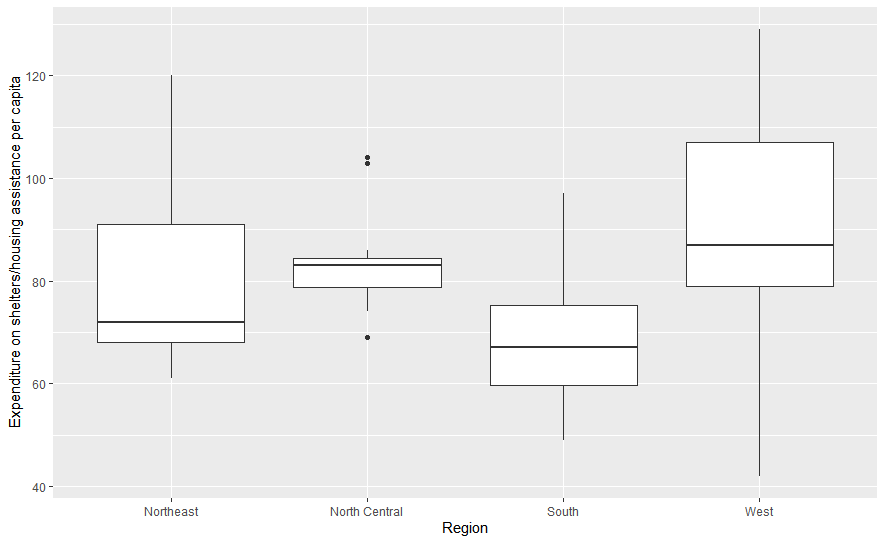
\includegraphics[width=\textwidth]{PS1_Plot2}
	\caption{Per capita expenditure per region}
	\label{fig:regionplot}
\end{figure}

\subsection{Task 3}
\textit{Please plot the relationship between \emph{Y} and \emph{X1}? Describe this graph and the relationship. Reproduce the above graph including one more variable \emph{Region} and display different regions with different types of symbols and colors.}
\vspace{0.5cm}

For the third task, I plotted the correlation between expenditures for shelters and housing assistance (Y), and personal income per capita (X1), separated by region. I have added individual regression lines for each region, in the same colour as the region’s observations. 

\lstinputlisting[language=R, firstline=62, lastline=66]{PS01_DW_R.R}

\begin{figure}[h]
	\centering
	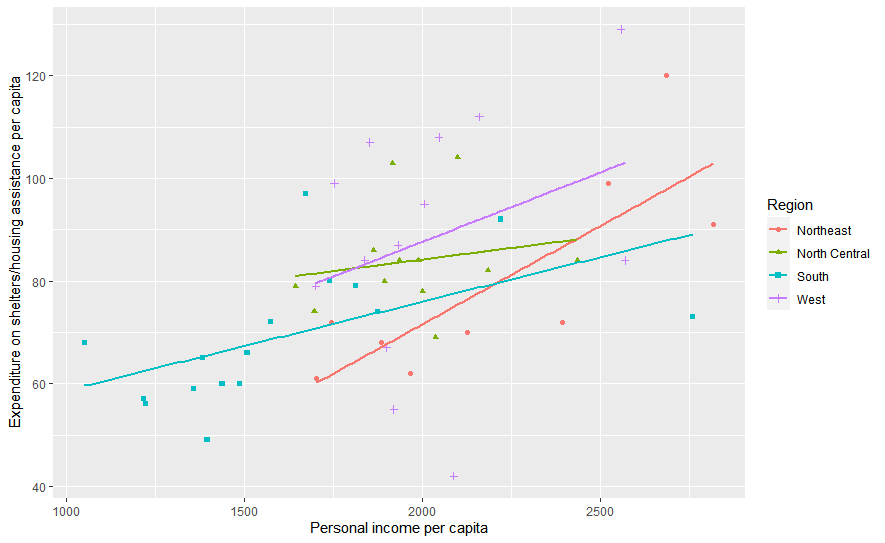
\includegraphics[width=\textwidth]{PS1_Plot3}
	\caption{Per capita expenditure per region}
	\label{fig:reg_x1_plot}
\end{figure}


In Figure \ref{fig:reg_x1_plot}, we can again see the higher level of expenditure in the West (purple). Furthermore, we see that the correlation of Y and X1 is largest in the Northeastern region (red), and smallest in the North-Central region (green). We also can see that all of the states with the lowest personal income per capita; as well as most of the states with low expenditures (Y) are located in the South. Expenditures in this region are overall low, leading to a weaker effect compared to the Northeast or the West. Finally, we can see that there are a few observations in the Western region with uncharacteristically low values for Y; likely, these observations diminish the size of the effect in the West somewhat.


\end{document}